\documentclass[10pt,twocolumn]{article}
\usepackage[margin=0.75in]{geometry}
\usepackage{graphicx}
\usepackage{booktabs}
\usepackage{amsmath,amssymb}
\usepackage{hyperref}
\usepackage{caption}
\usepackage{subcaption}
\usepackage[table]{xcolor}
\usepackage{enumitem}
\usepackage{float}
\usepackage{titlesec}

\setlength{\parskip}{3pt}
\setlength{\columnsep}{0.25in}
\setlist{nosep,leftmargin=1.2em}
\graphicspath{{../imgs/}}
\captionsetup{font=small,labelfont=bf,skip=4pt}
\titlespacing*{\section}{0pt}{8pt}{4pt}
\titlespacing*{\subsection}{0pt}{6pt}{3pt}

\title{\vspace{-1.8em}\textbf{Dual-Core Machine Learning Accelerator
for Attention Mechanism}\vspace{-0.8em}}
\author{Yufan Wang, Purab Balani, Jasmine Le, Dennis Zang\\
The Best ECE260B Group -- Winter UCSD}
\date{}

\begin{document}
\maketitle

% ---------------------------------------------------------------
\section{Introduction}
% ---------------------------------------------------------------

The attention mechanism has become the fundamental computational
primitive in modern Transformer-based AI systems, enabling parallel
processing of global dependencies across input sequences. The core
operation, $A = QK^T$, requires pairwise interactions between all
elements, resulting in quadratic complexity with respect to sequence
length. As models scale to longer contexts, this computation becomes
the primary bottleneck in both training and inference.

This project addresses these challenges by designing a custom
hardware accelerator in TSMC 65\,nm targeting 1\,GHz. The design
progresses from a single-core baseline through hierarchical
synthesis, dual-core integration with asynchronous clock-domain
crossing, pipelined multiplier optimization, and sparsity-aware
gating. The goals are to improve throughput through parallelism,
reduce energy via sparsity, and optimize memory access patterns
for scalable deployment.

% ---------------------------------------------------------------
\section{Problem Formulation}
% ---------------------------------------------------------------

Given query matrix $Q$ and key matrix $K$ with 8-bit signed
elements, the accelerator computes the attention score matrix:

\vspace{-4pt}
$$A_{ij} = Q_i \cdot K_j
= \sum_{k=0}^{7} Q_i[k] \cdot K_j[k]$$
\vspace{-4pt}

Each row is then normalized via $L_1$ normalization:

\vspace{-4pt}
$$\hat{A}_{ij}
= \frac{|A_{ij}|}{\sum_{j=0}^{N-1} |A_{ij}|}$$
\vspace{-4pt}

For the dual-core extension with 16 key vectors, the denominator
requires contributions from both cores:

\vspace{-4pt}
$$\sum_{j=0}^{15} |A_{ij}|
= \underbrace{\sum_{j=0}^{7} |A_{ij}|}_{\text{core0}}
+ \underbrace{\sum_{j=8}^{15} |A_{ij}|}_{\text{core1}}$$
\vspace{-4pt}

This introduces inter-core communication for normalization across
independent clock domains.

% ---------------------------------------------------------------
\section{Technical Approach}
% ---------------------------------------------------------------

\subsection{Single-Core Architecture (Steps 1--2)}

The base design implements a modular single-core accelerator:
\begin{itemize}
  \item \textbf{MAC Array} (\texttt{mac\_array}): 8
    \texttt{mac\_col} instances with pipelined adder trees
    ($\lceil\log_2 8\rceil = 3$ stages). Query vectors propagate
    systolically; Key vectors are pre-loaded.
  \item \textbf{SRAMs}: \texttt{qmem} (64b$\times$16),
    \texttt{kmem} (64b$\times$16), \texttt{pmem} (160b$\times$16)
    for input/output storage.
  \item \textbf{OFIFO}: output FIFO buffering MAC results.
  \item \textbf{Normalizer} (\texttt{sfp\_row}): sequential
    row-wise $L_1$ normalization via non-restoring division,
    producing 10-bit outputs. Division is the most timing-critical
    operation and dominates the critical path.
\end{itemize}

Each cycle computes one full row:
$[Q_i K_0,\; Q_i K_1,\; \ldots,\; Q_i K_7]$.

\begin{figure}[H]
  \centering
  \begin{subfigure}{0.48\linewidth}
    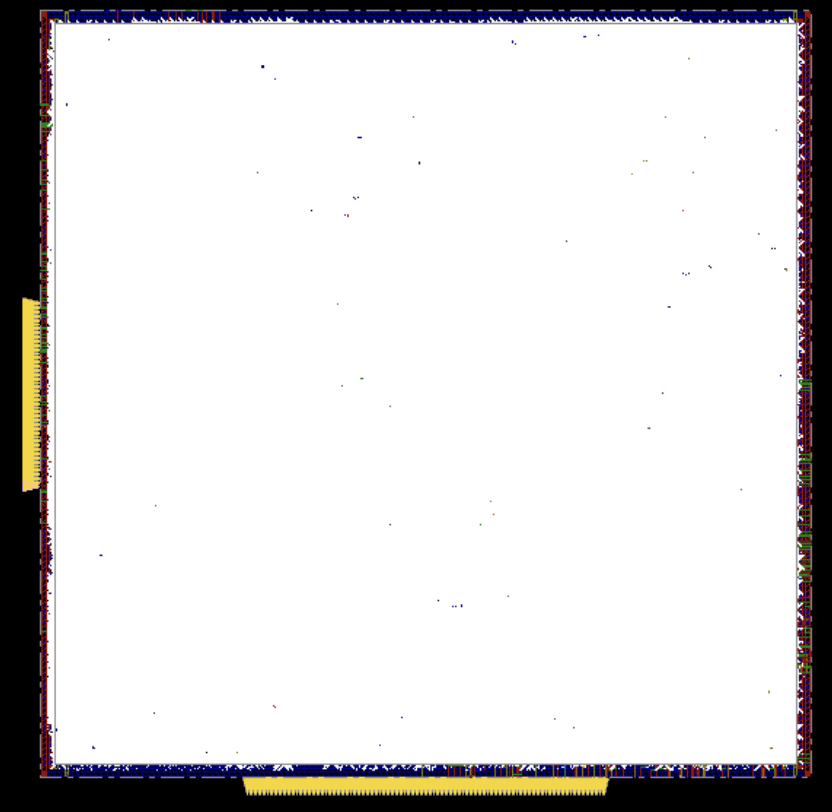
\includegraphics[width=\linewidth]{Step1_pnr.png}
    \caption{Step 1 flat PnR layout}
  \end{subfigure}
  \hfill
  \begin{subfigure}{0.48\linewidth}
    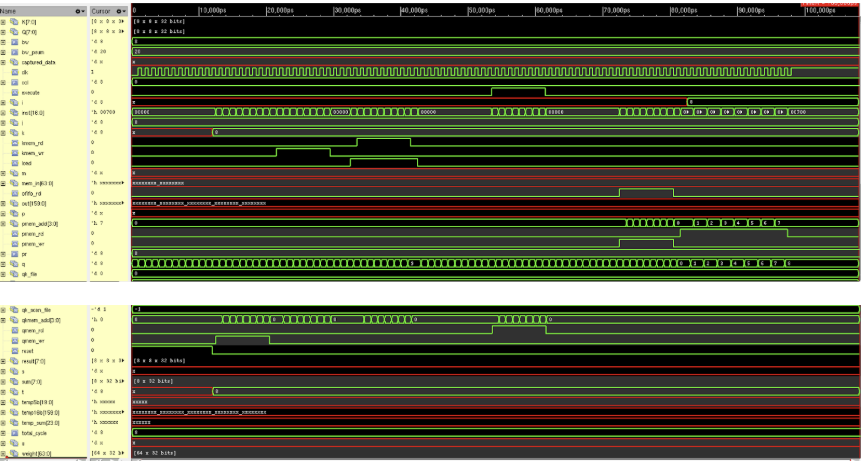
\includegraphics[width=\linewidth]{Step1_vcd.png}
    \caption{Step 1 MAC output VCD}
  \end{subfigure}
  \\[4pt]
  \begin{subfigure}{0.96\linewidth}
    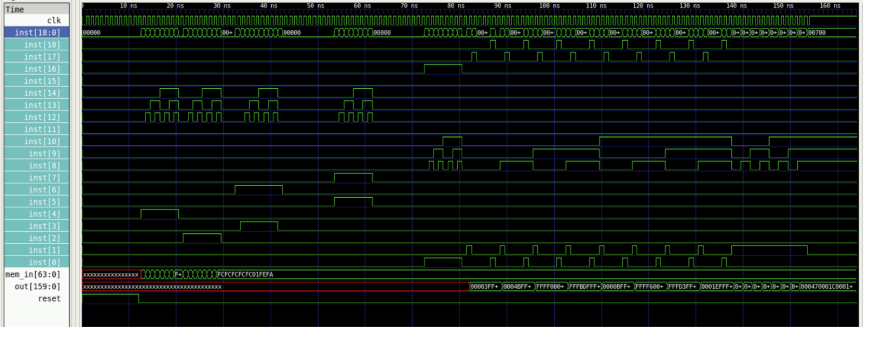
\includegraphics[width=\linewidth]{Step2_vcd.png}
    \caption{Step 2 normalization VCD}
  \end{subfigure}
  \caption{Steps 1--2: PnR layout, MAC functional verification,
    and normalization output matching expected results.}
  \label{fig:step12}
\end{figure}

\subsection{Hierarchical Synthesis (Step 3)}

To enable scalable physical design, SRAMs are synthesized and
placed independently as hard macros (top metal M4, 4\,$\mu$m pin
pitch), then integrated into the core via hierarchical PnR (Place
and Route). This improves routing efficiency and timing closure
by isolating SRAM routing from standard-cell logic.

\textbf{Design choice.} \texttt{kmem}/\texttt{qmem} are placed
near input ports (left edge); \texttt{pmem} near output ports
(bottom), minimizing wire delay on critical data paths.

Result: \textbf{WNS = +0.103\,ns}, 45,972 instances,
632,212\,$\mu$m$^2$, 0 DRC/LVS violations.

\begin{figure}[H]
  \centering
  \begin{subfigure}{0.44\linewidth}
    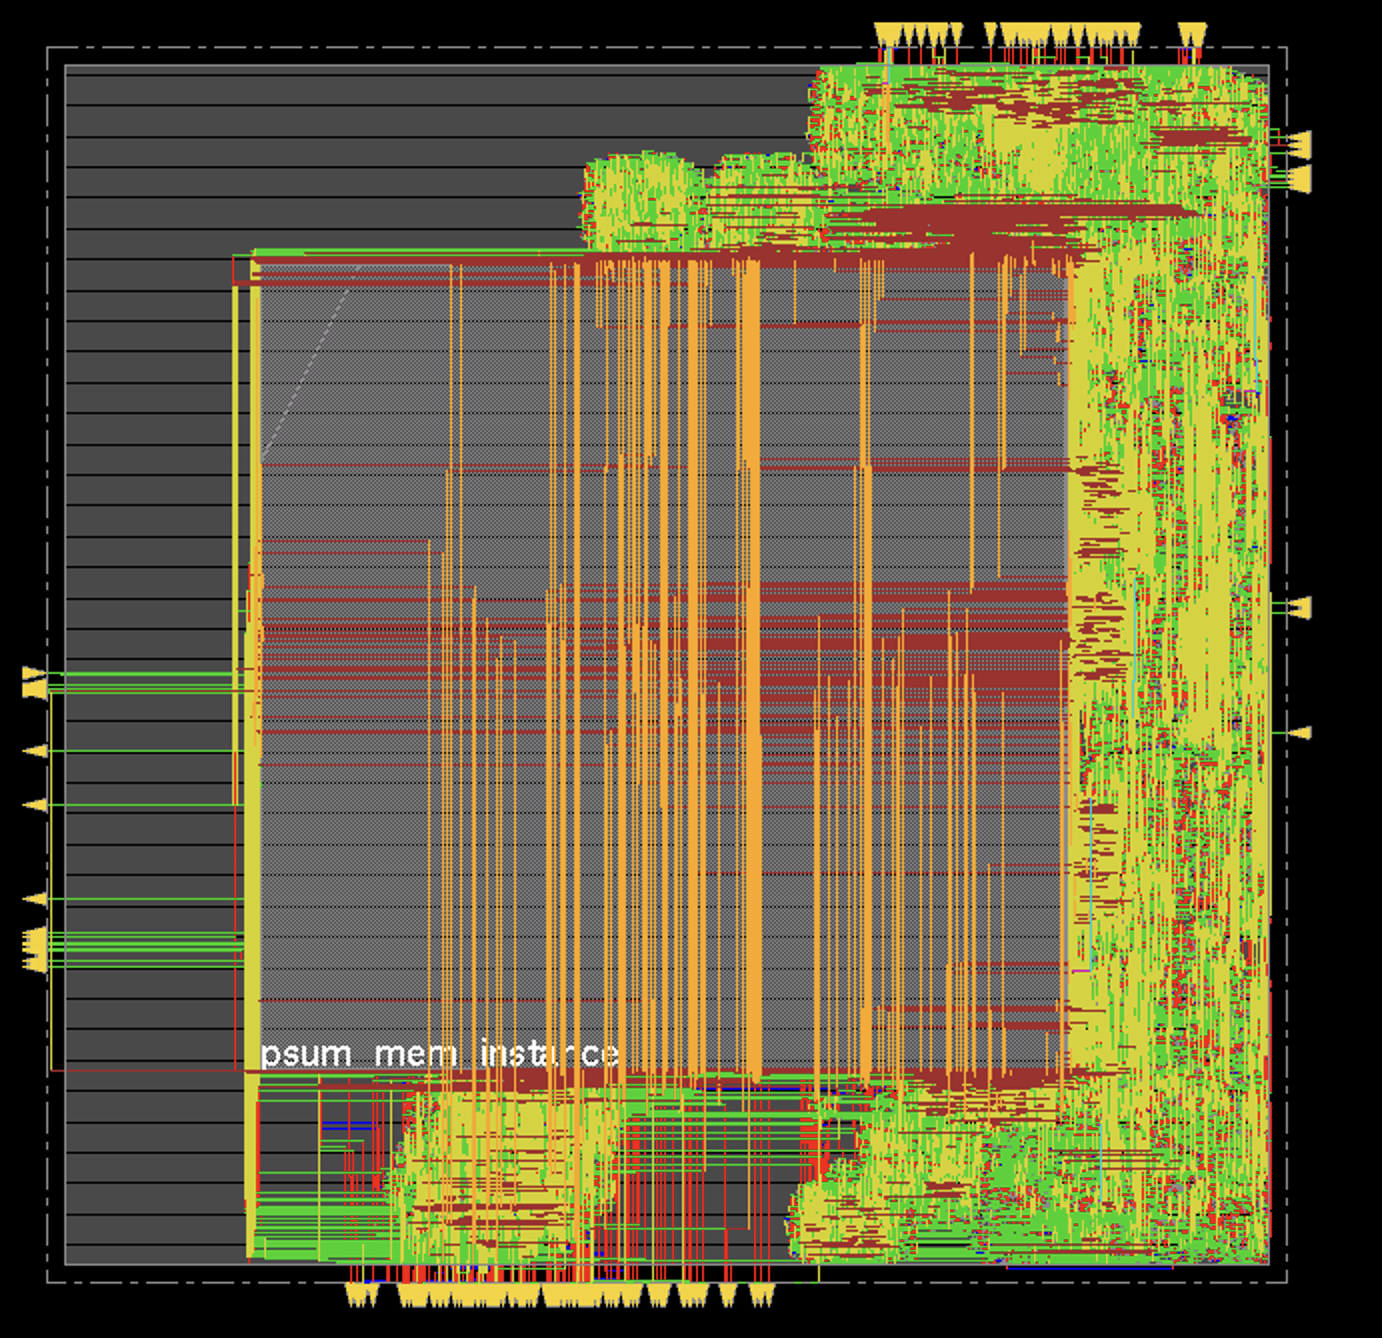
\includegraphics[width=\linewidth]{Step3_PnR.png}
    \caption{Hierarchical layout}
  \end{subfigure}
  \hfill
  \begin{subfigure}{0.52\linewidth}
    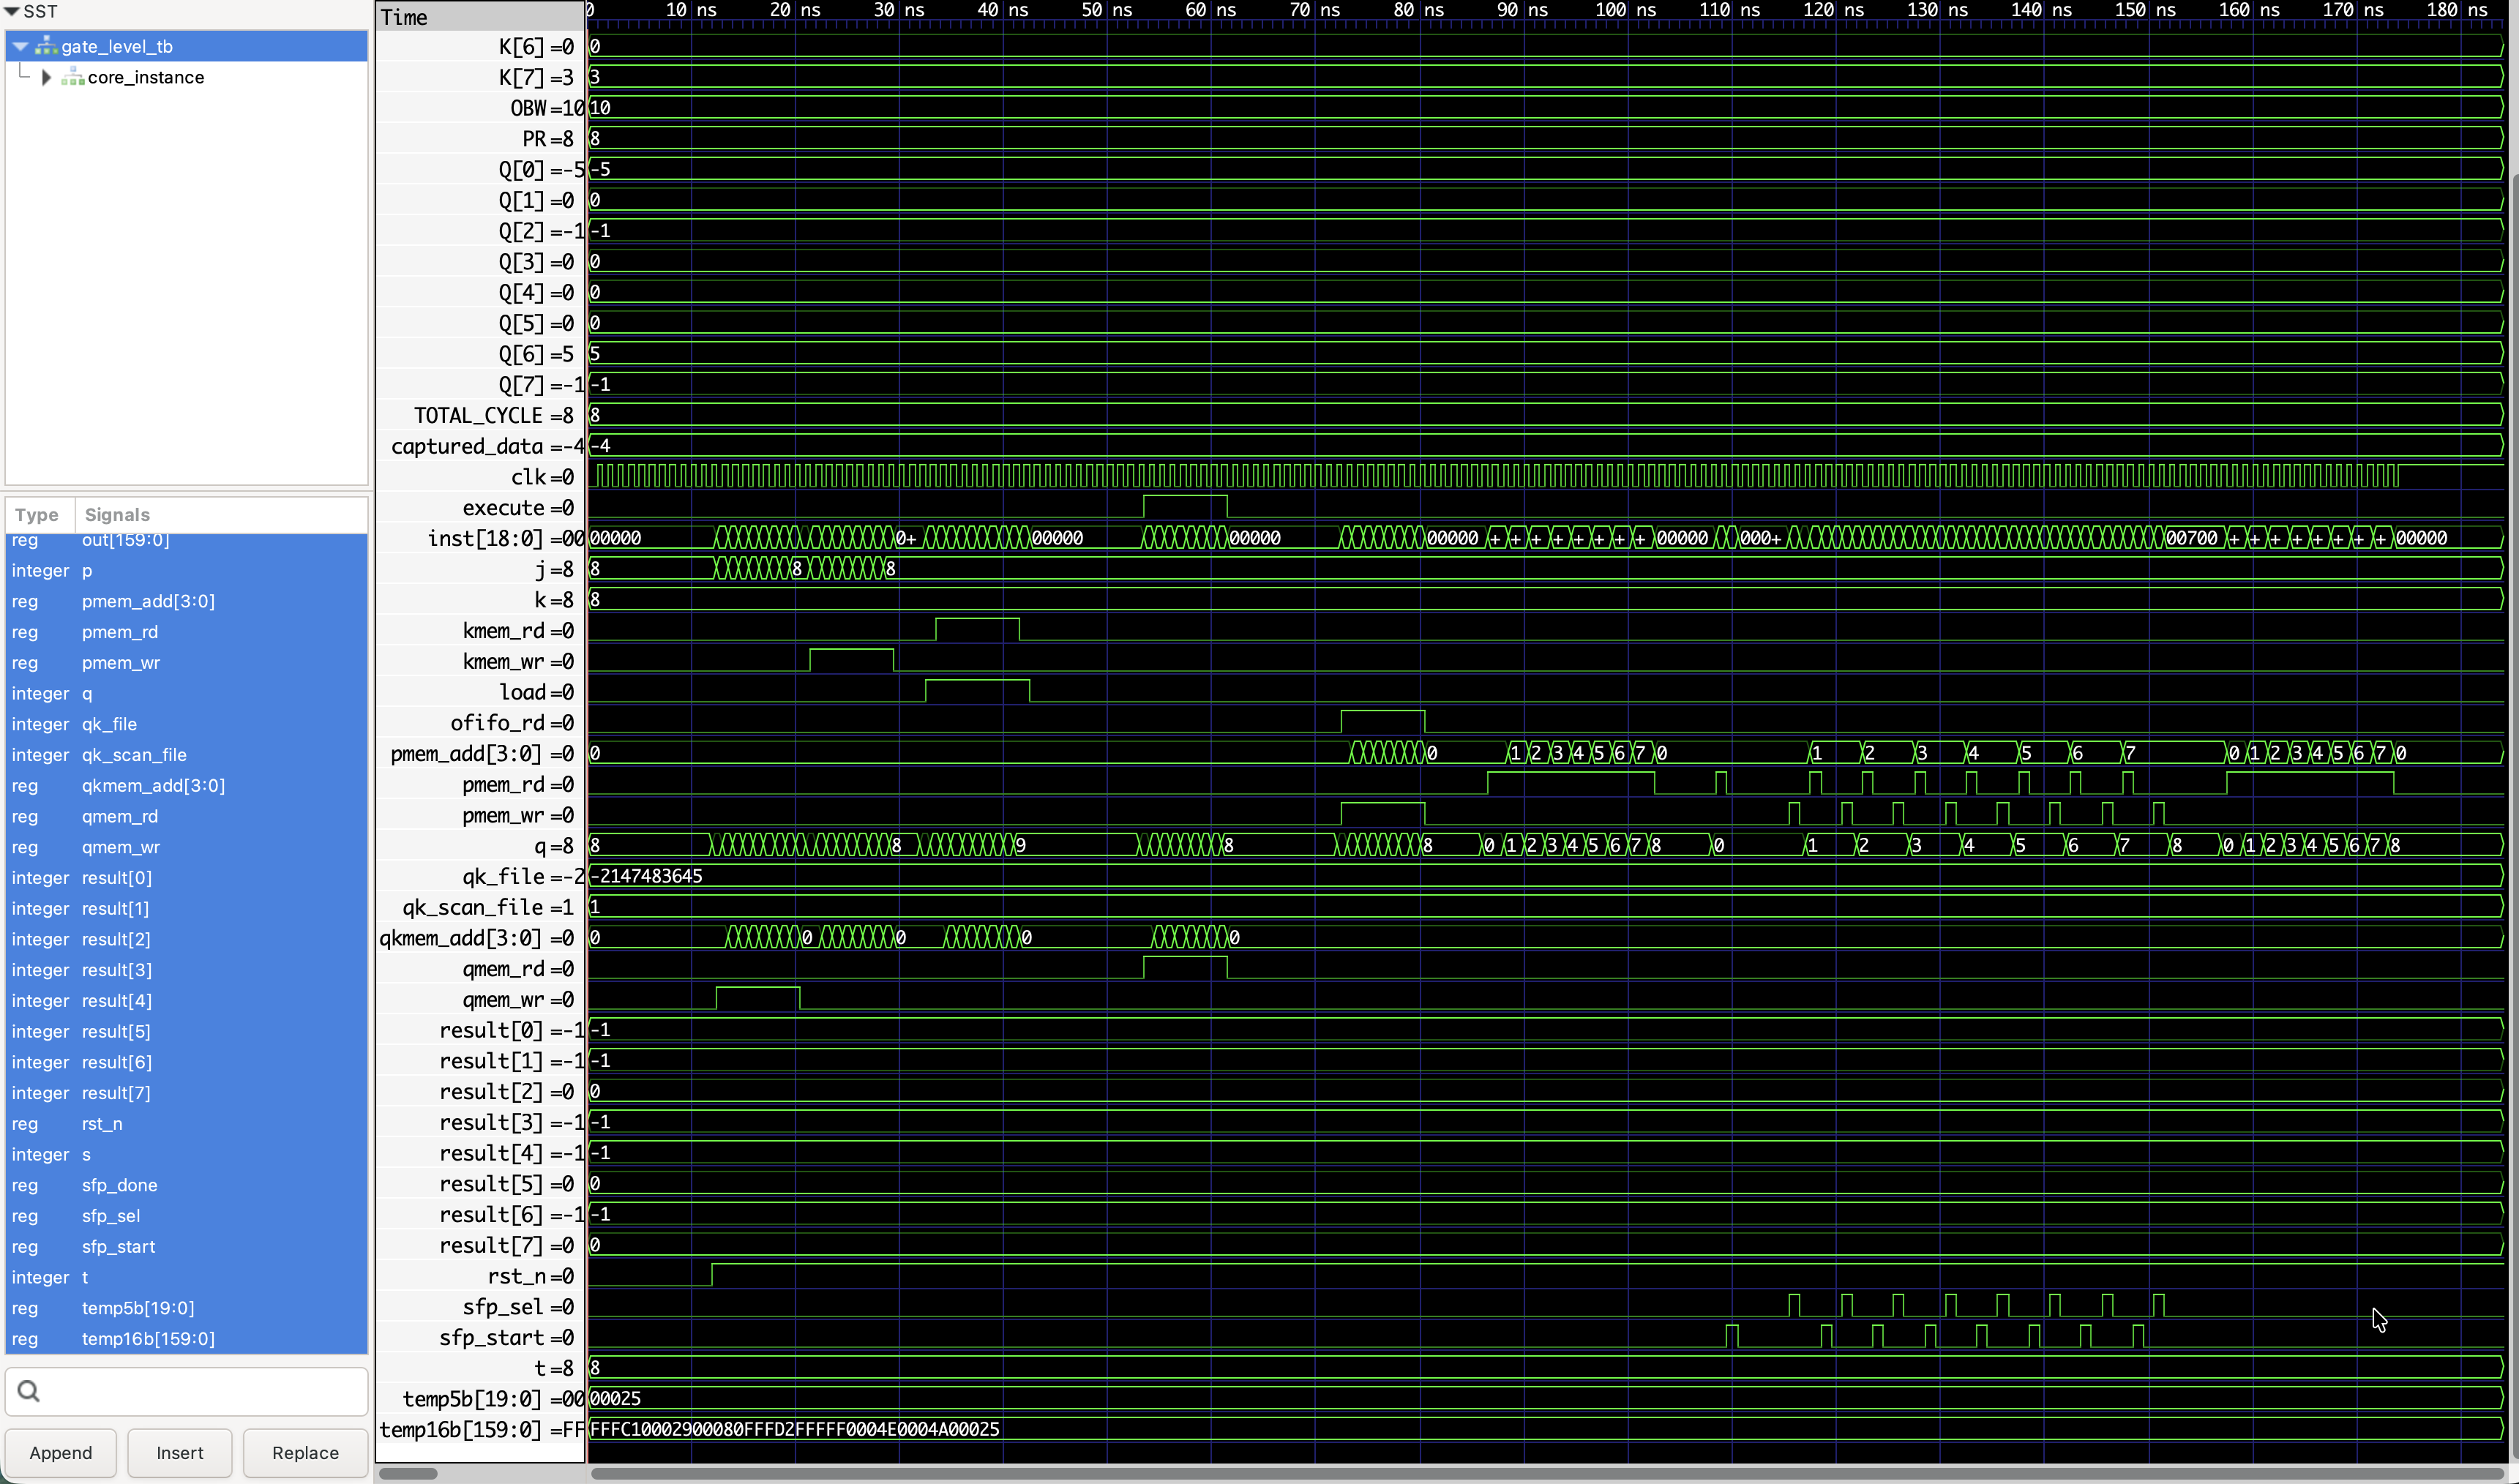
\includegraphics[width=\linewidth]{Step3_vcd.png}
    \caption{Gate-level simulation}
  \end{subfigure}
  \caption{Step 3: SRAM macros visible as rectangular blocks.
    Gate-level sim confirms post-synthesis correctness.}
  \label{fig:step3}
\end{figure}

\subsection{Dual-Core Architecture (Step 4)}

Two identical cores operate on independent clock domains
(\texttt{clk0}=1\,GHz, \texttt{clk1}=800\,MHz), each processing
8 of the 16 key vectors in parallel.

\textbf{Key challenge.} Normalization requires a global sum across
both cores operating in different clock domains.

\textbf{Solution --- MUX-based bus synchronizer.} A 2-stage FF
synchronizer qualifies the valid signal; a MUX captures the
multi-bit sum data only when valid is asserted in the destination
domain. This was chosen over a full async FIFO for simplicity and
low latency ($\sim$3 destination clock cycles).

\textbf{Execution flow:} (1) Both cores compute partial dot
products simultaneously. (2) Partial sums exchanged via CDC.
(3) Combined normalization performed independently.

Result: \textbf{WNS = +0.098\,ns}, 167,896 instances,
623,612\,$\mu$m$^2$, 0 DRC/LVS.

\begin{figure}[H]
  \centering
  \begin{subfigure}{0.44\linewidth}
    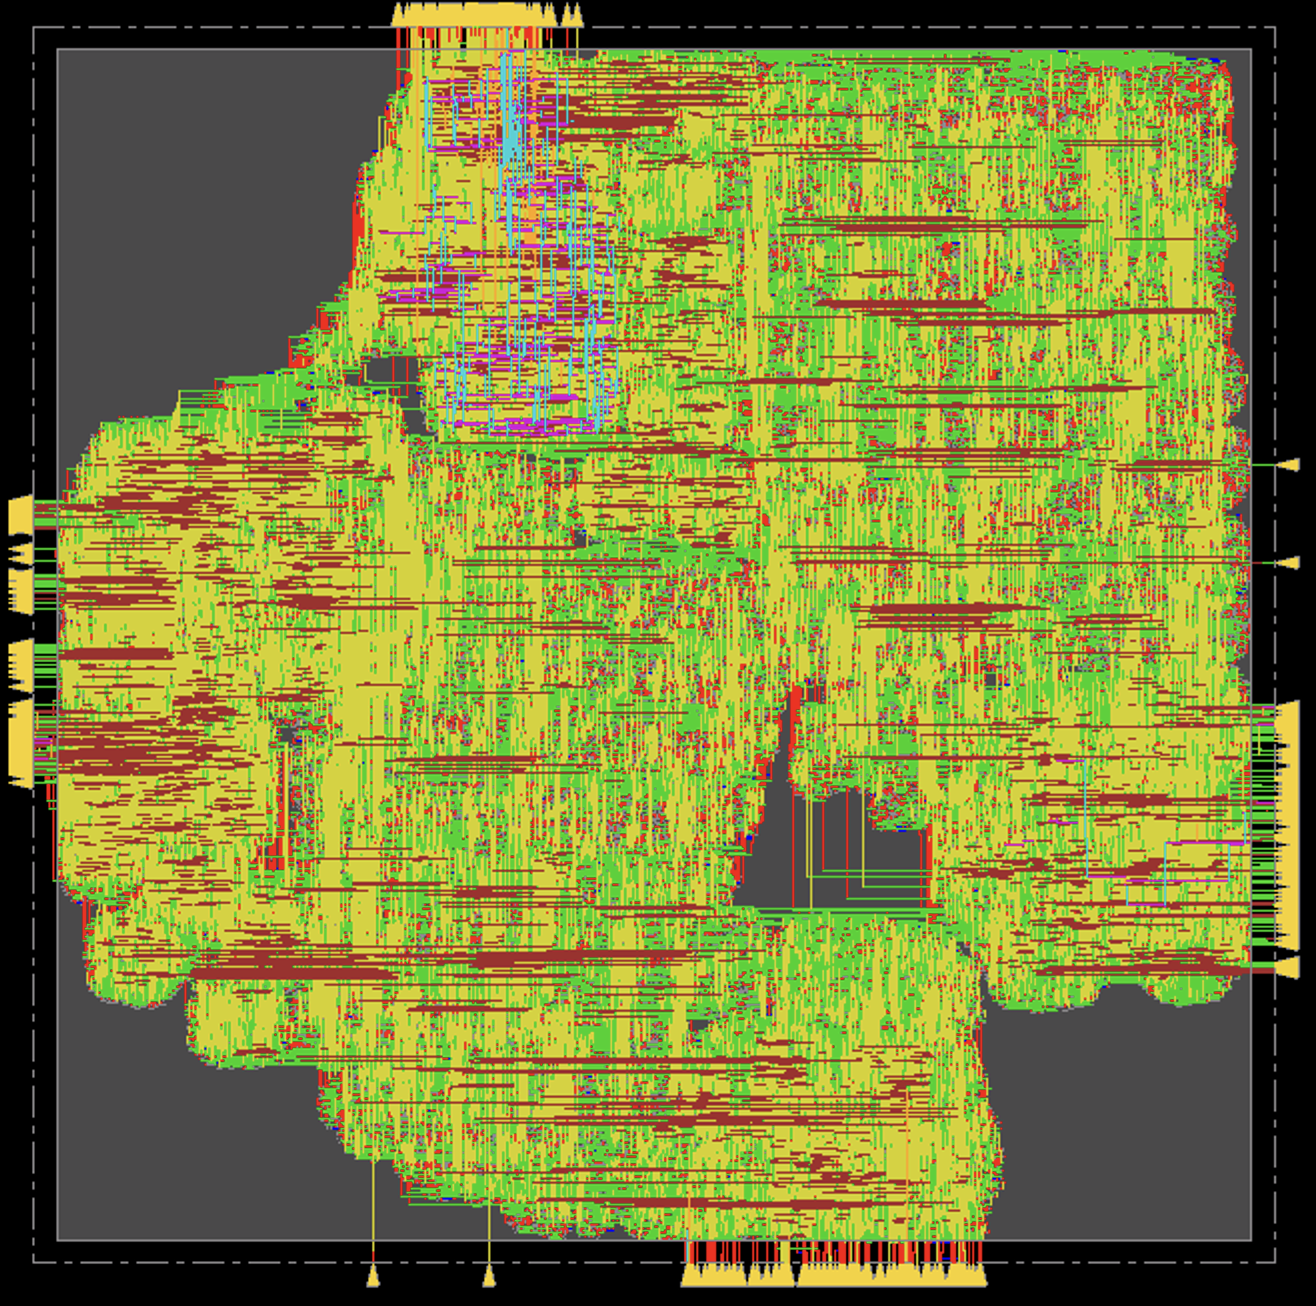
\includegraphics[width=\linewidth]{Step4_PnR.png}
    \caption{Dual-core fullchip layout}
  \end{subfigure}
  \hfill
  \begin{subfigure}{0.52\linewidth}
    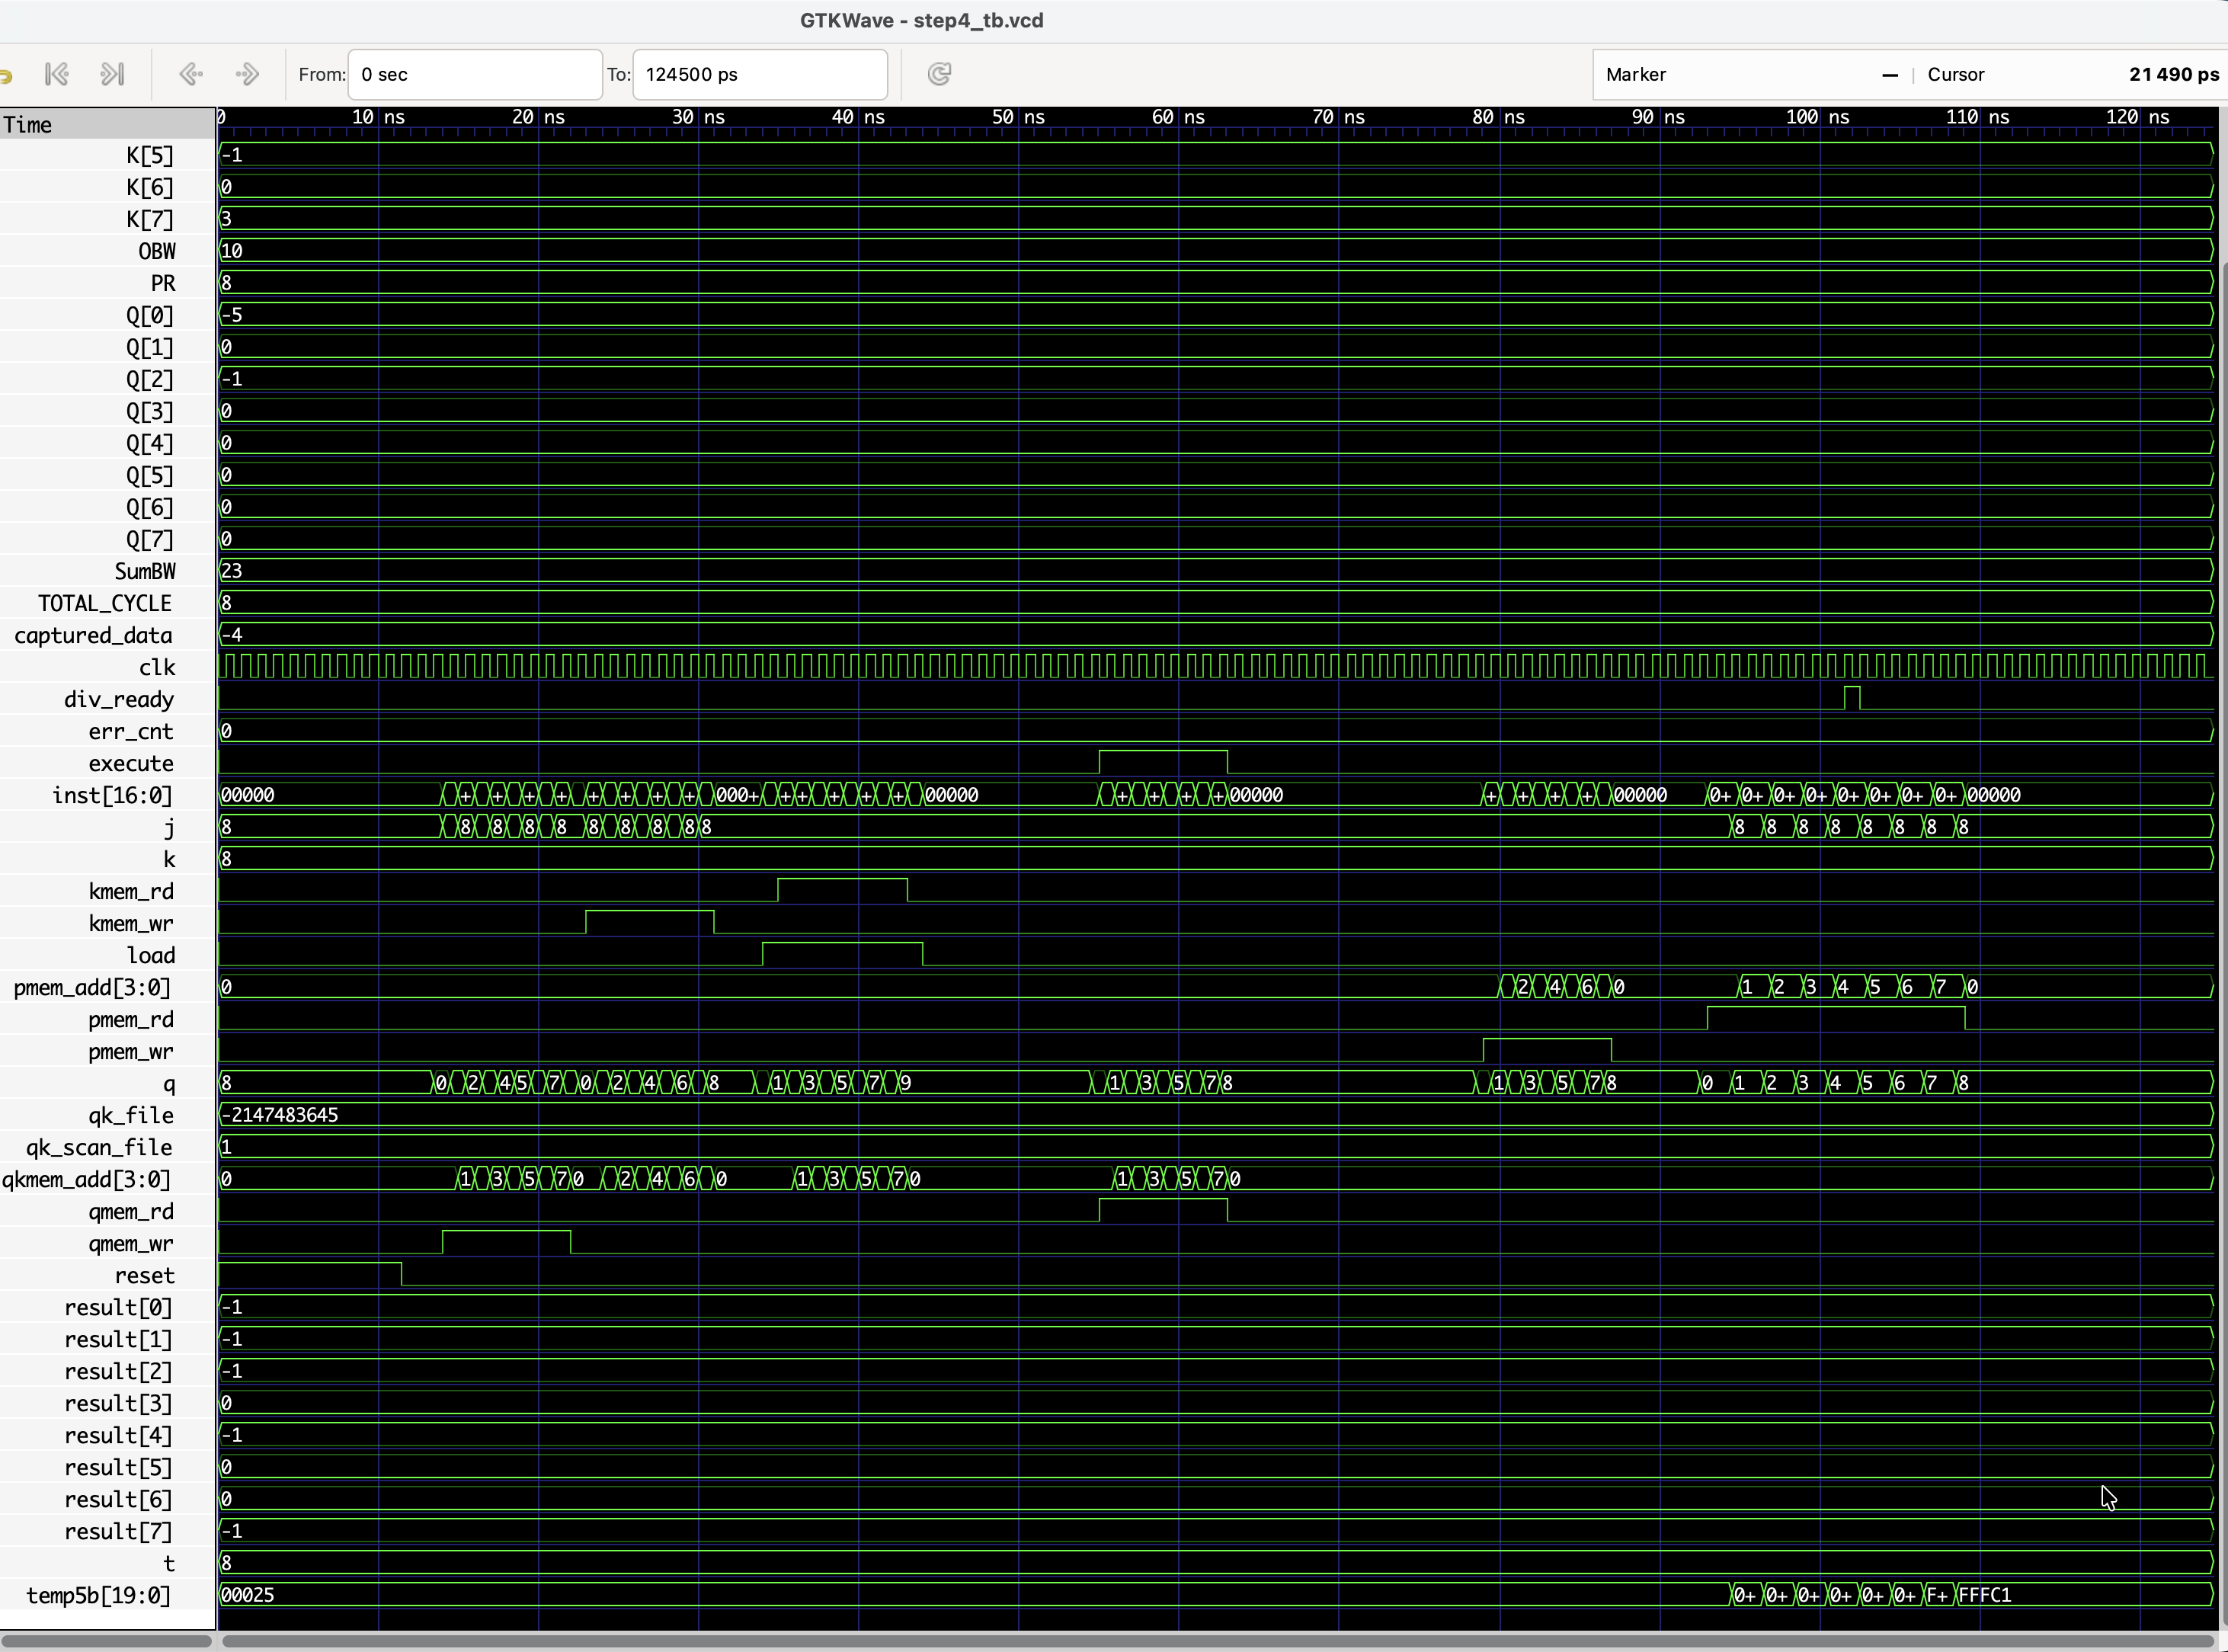
\includegraphics[width=\linewidth]{Step4_Sim.png}
    \caption{Dual-core simulation}
  \end{subfigure}
  \caption{Step 4: dual-core PnR (167,896 instances) and
    functional verification with CDC sum exchange.}
  \label{fig:step4}
\end{figure}

\subsection{Pipelined Multiplier Optimization (Step 5)}

\textbf{Motivation.} The 8-bit$\times$8-bit multiplier is the
widest combinational block in the MAC datapath, consuming most of
the timing budget at 1\,GHz.

\textbf{Approach.} An input-register stage is inserted before the
multiplier, enabling \texttt{compile\_ultra -retime} to
redistribute combinational logic across pipeline boundaries. This
breaks the critical multiply path without changing functionality.

\textbf{Why this pipeline cut?} Placing the register \emph{before}
(rather than after) the multiplier gives the retiming engine maximum
flexibility to pull partial-product logic forward or push
adder-tree logic backward, balancing stage delays automatically.

Result: post-synthesis WNS = 0.00\,ns; post-PnR
\textbf{WNS = +0.023\,ns}. All 8 test cycles pass.

\begin{figure}[H]
  \centering
  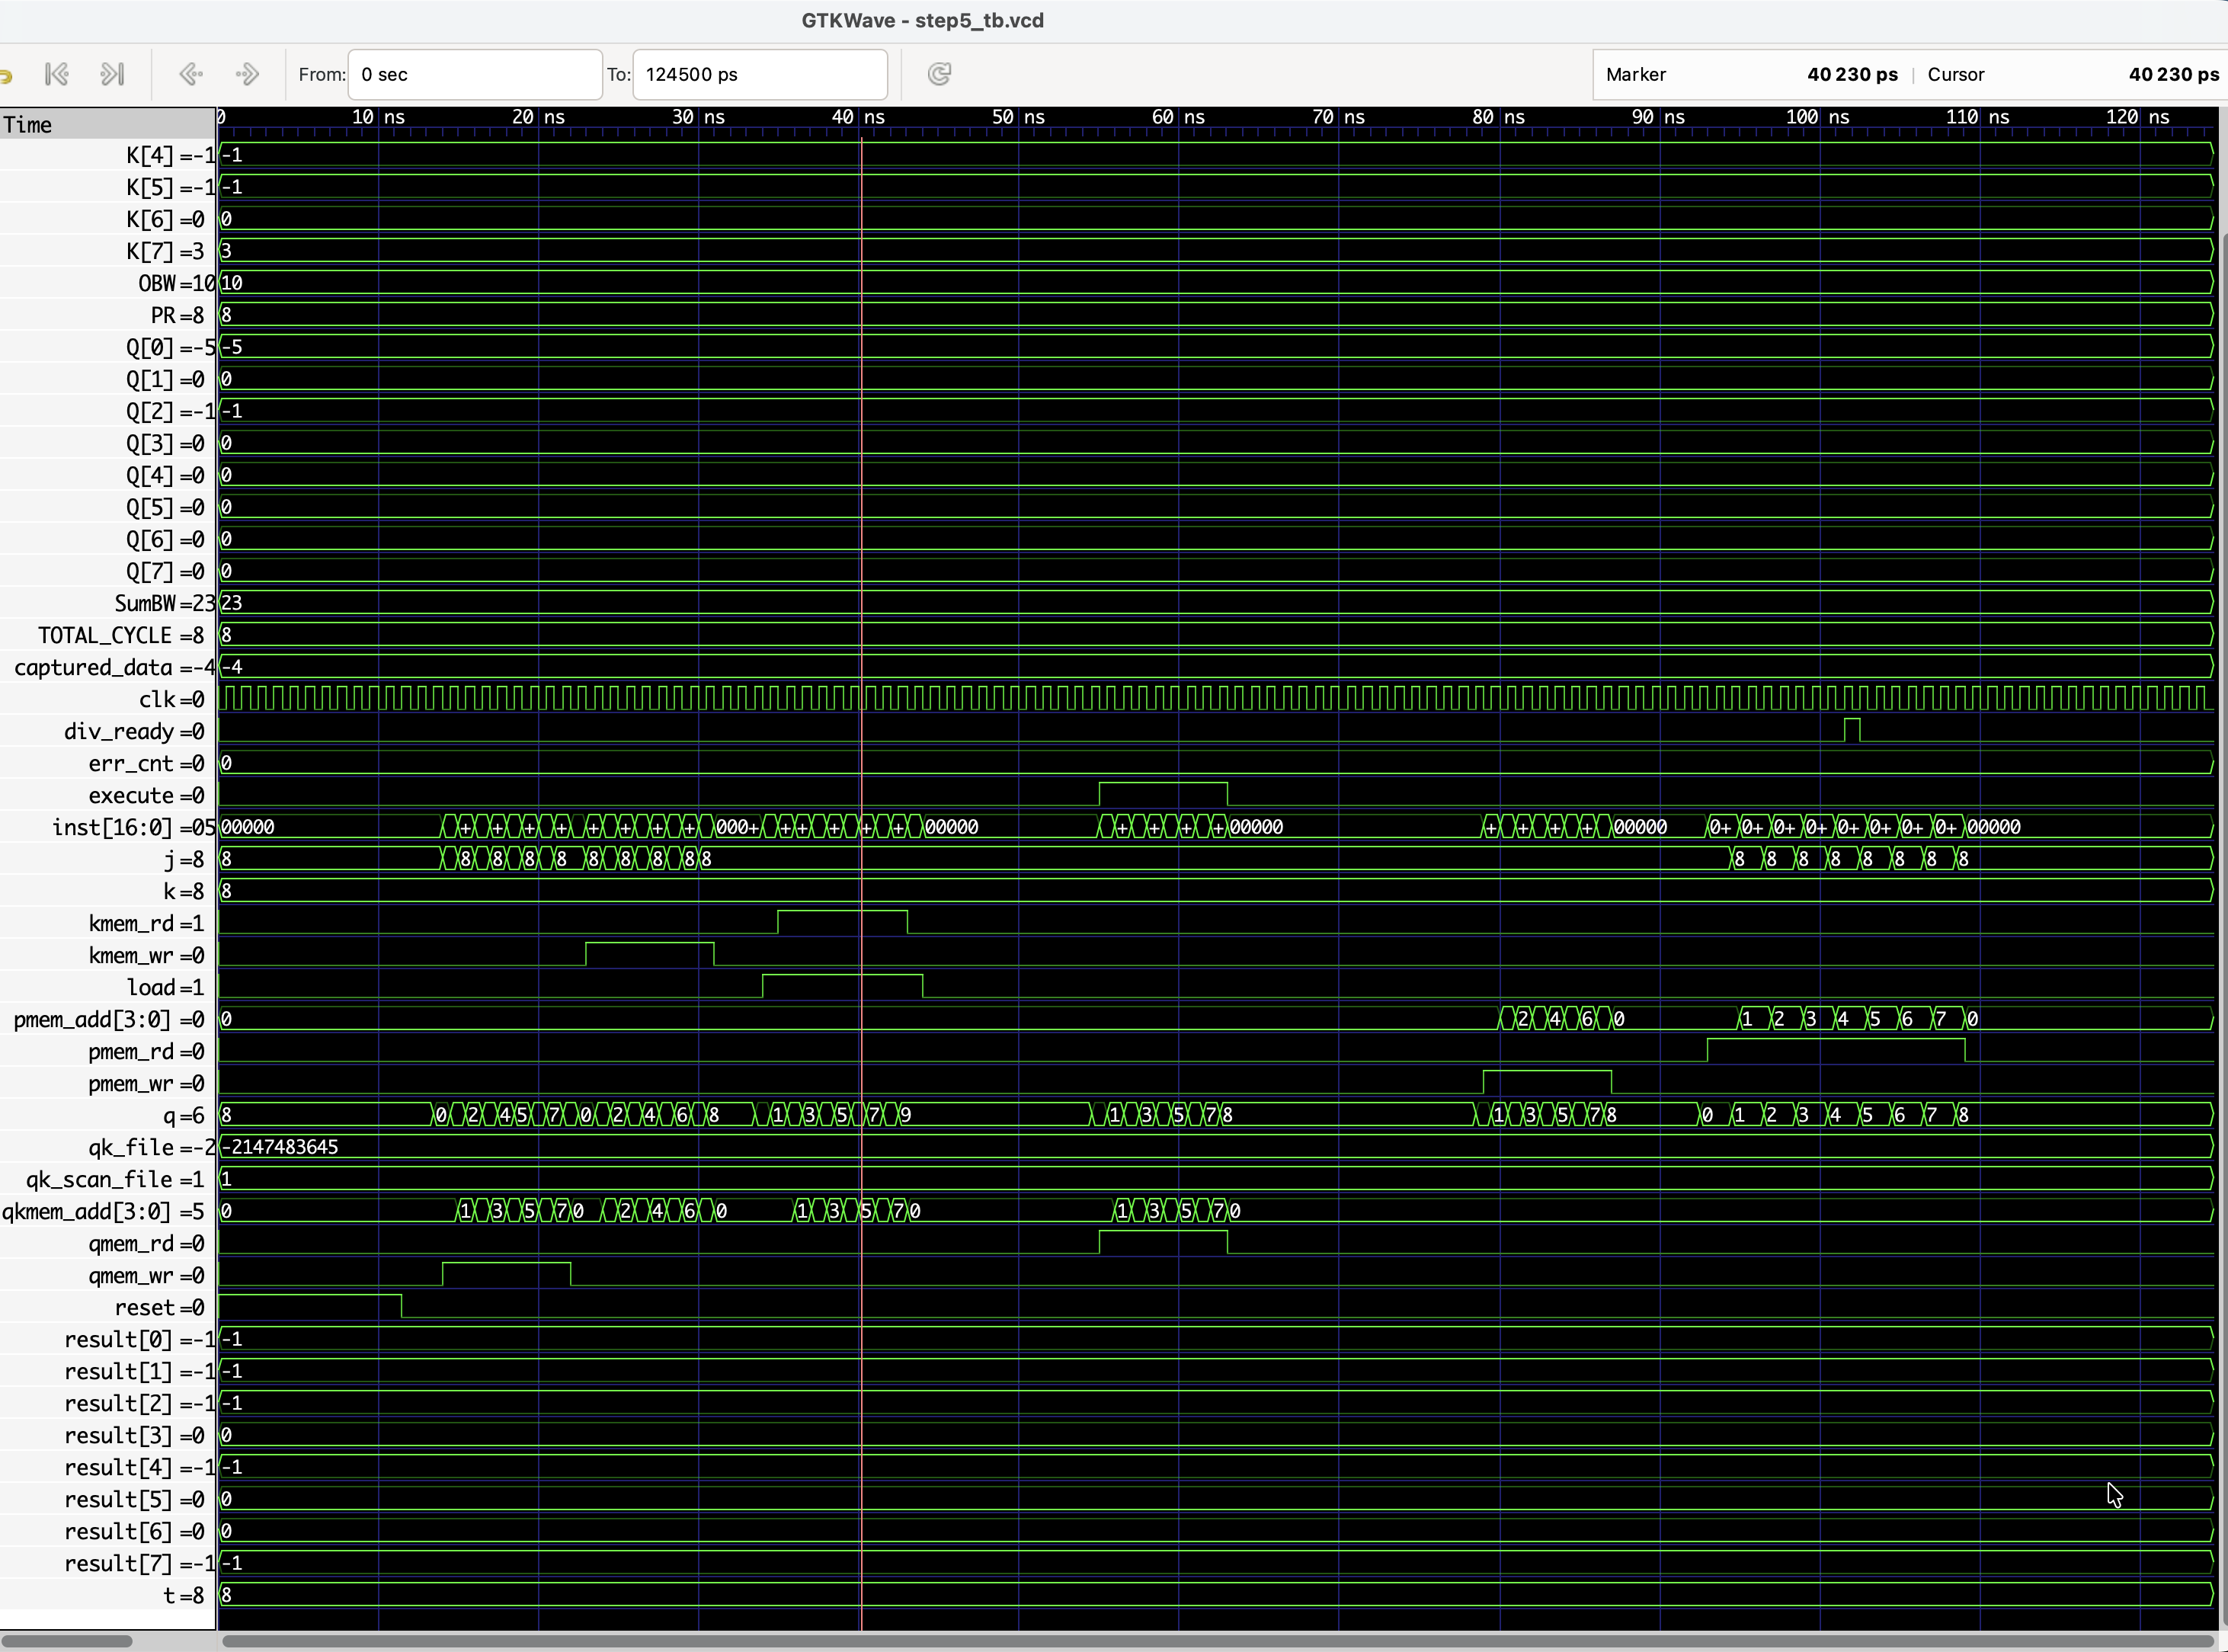
\includegraphics[width=\linewidth]{Step5_vcd.png}
  \caption{Step 5: pipelined MAC verification --- all 8
    query vectors produce correct $Q \times K$ outputs.}
  \label{fig:step5}
\end{figure}

\subsection{Two-Stage Multiplier \& Sparsity (Step 6)}

\textbf{Two-stage pipelined multiplier.}
The 8-bit multiply is explicitly split into two pipeline stages:
\begin{enumerate}
  \item \textbf{Cycle 1 --- Half-width multiplies:}
    $P_\text{lo} = a[3{:}0] \times b$,\;
    $P_\text{hi} = a[7{:}4] \times b$.
  \item \textbf{Cycle 2 --- Combine:}
    $\text{product} = P_\text{lo} + (P_\text{hi} \ll 4)$.
\end{enumerate}

\textbf{Why split at the 4-bit boundary?} This halves the
partial-product tree depth, reducing per-stage combinational delay
by $\sim$50\%. The combine stage (shift-and-add) is cheap. Total
MAC latency = $2 + 1 + \lceil\log_2 \text{PR}\rceil$ = 6 cycles.

\textbf{Sparsity-aware attention.} Attention matrices exhibit
inherent sparsity where many values contribute minimally to the
final result. Two levels of sparsity exploit this:

\textit{B1 --- Element-level gating.} If
$|Q_i K_j| < \theta_\text{elem}$, the output is gated to zero
via a MUX, suppressing downstream switching activity. Target:
$\sim$70\% sparsity.

\textit{B2 --- Row-level skipping.} If
$S_i = \sum_j |Q_i K_j| < \theta_\text{row}$, the entire
normalization stage is skipped, saving both power and clock cycles.
Target: $\sim$30\% sparsity.

The sparsity controller adds one comparator and MUX per column
($<$1\% area overhead).

Result: \textbf{WNS = +0.058\,ns}, 173,920 instances,
663,643\,$\mu$m$^2$, 0 DRC/LVS.

\begin{figure}[H]
  \centering
  \begin{subfigure}{0.44\linewidth}
    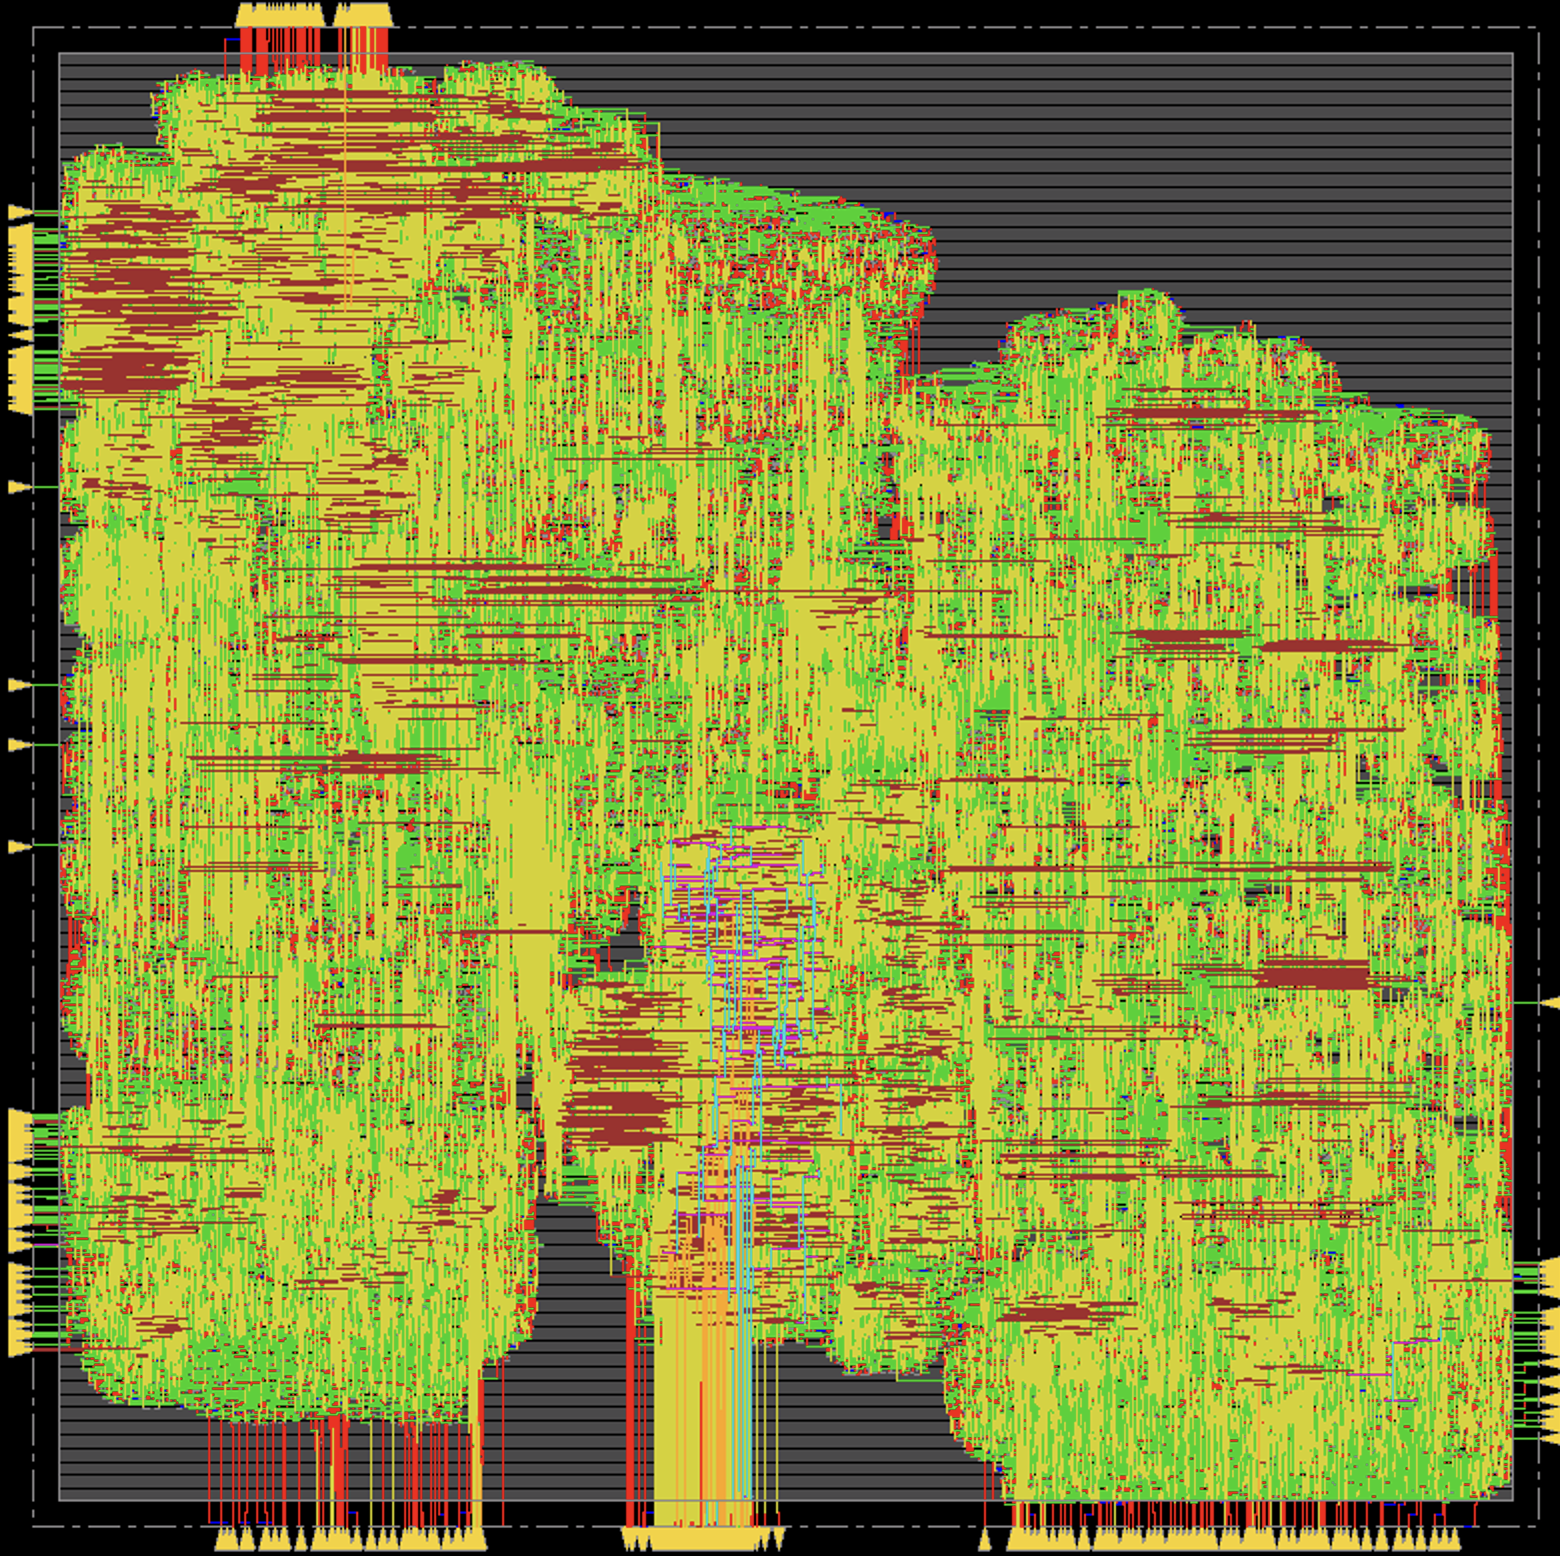
\includegraphics[width=\linewidth]{Step6_PnR.png}
    \caption{Step 6 final layout}
  \end{subfigure}
  \hfill
  \begin{subfigure}{0.52\linewidth}
    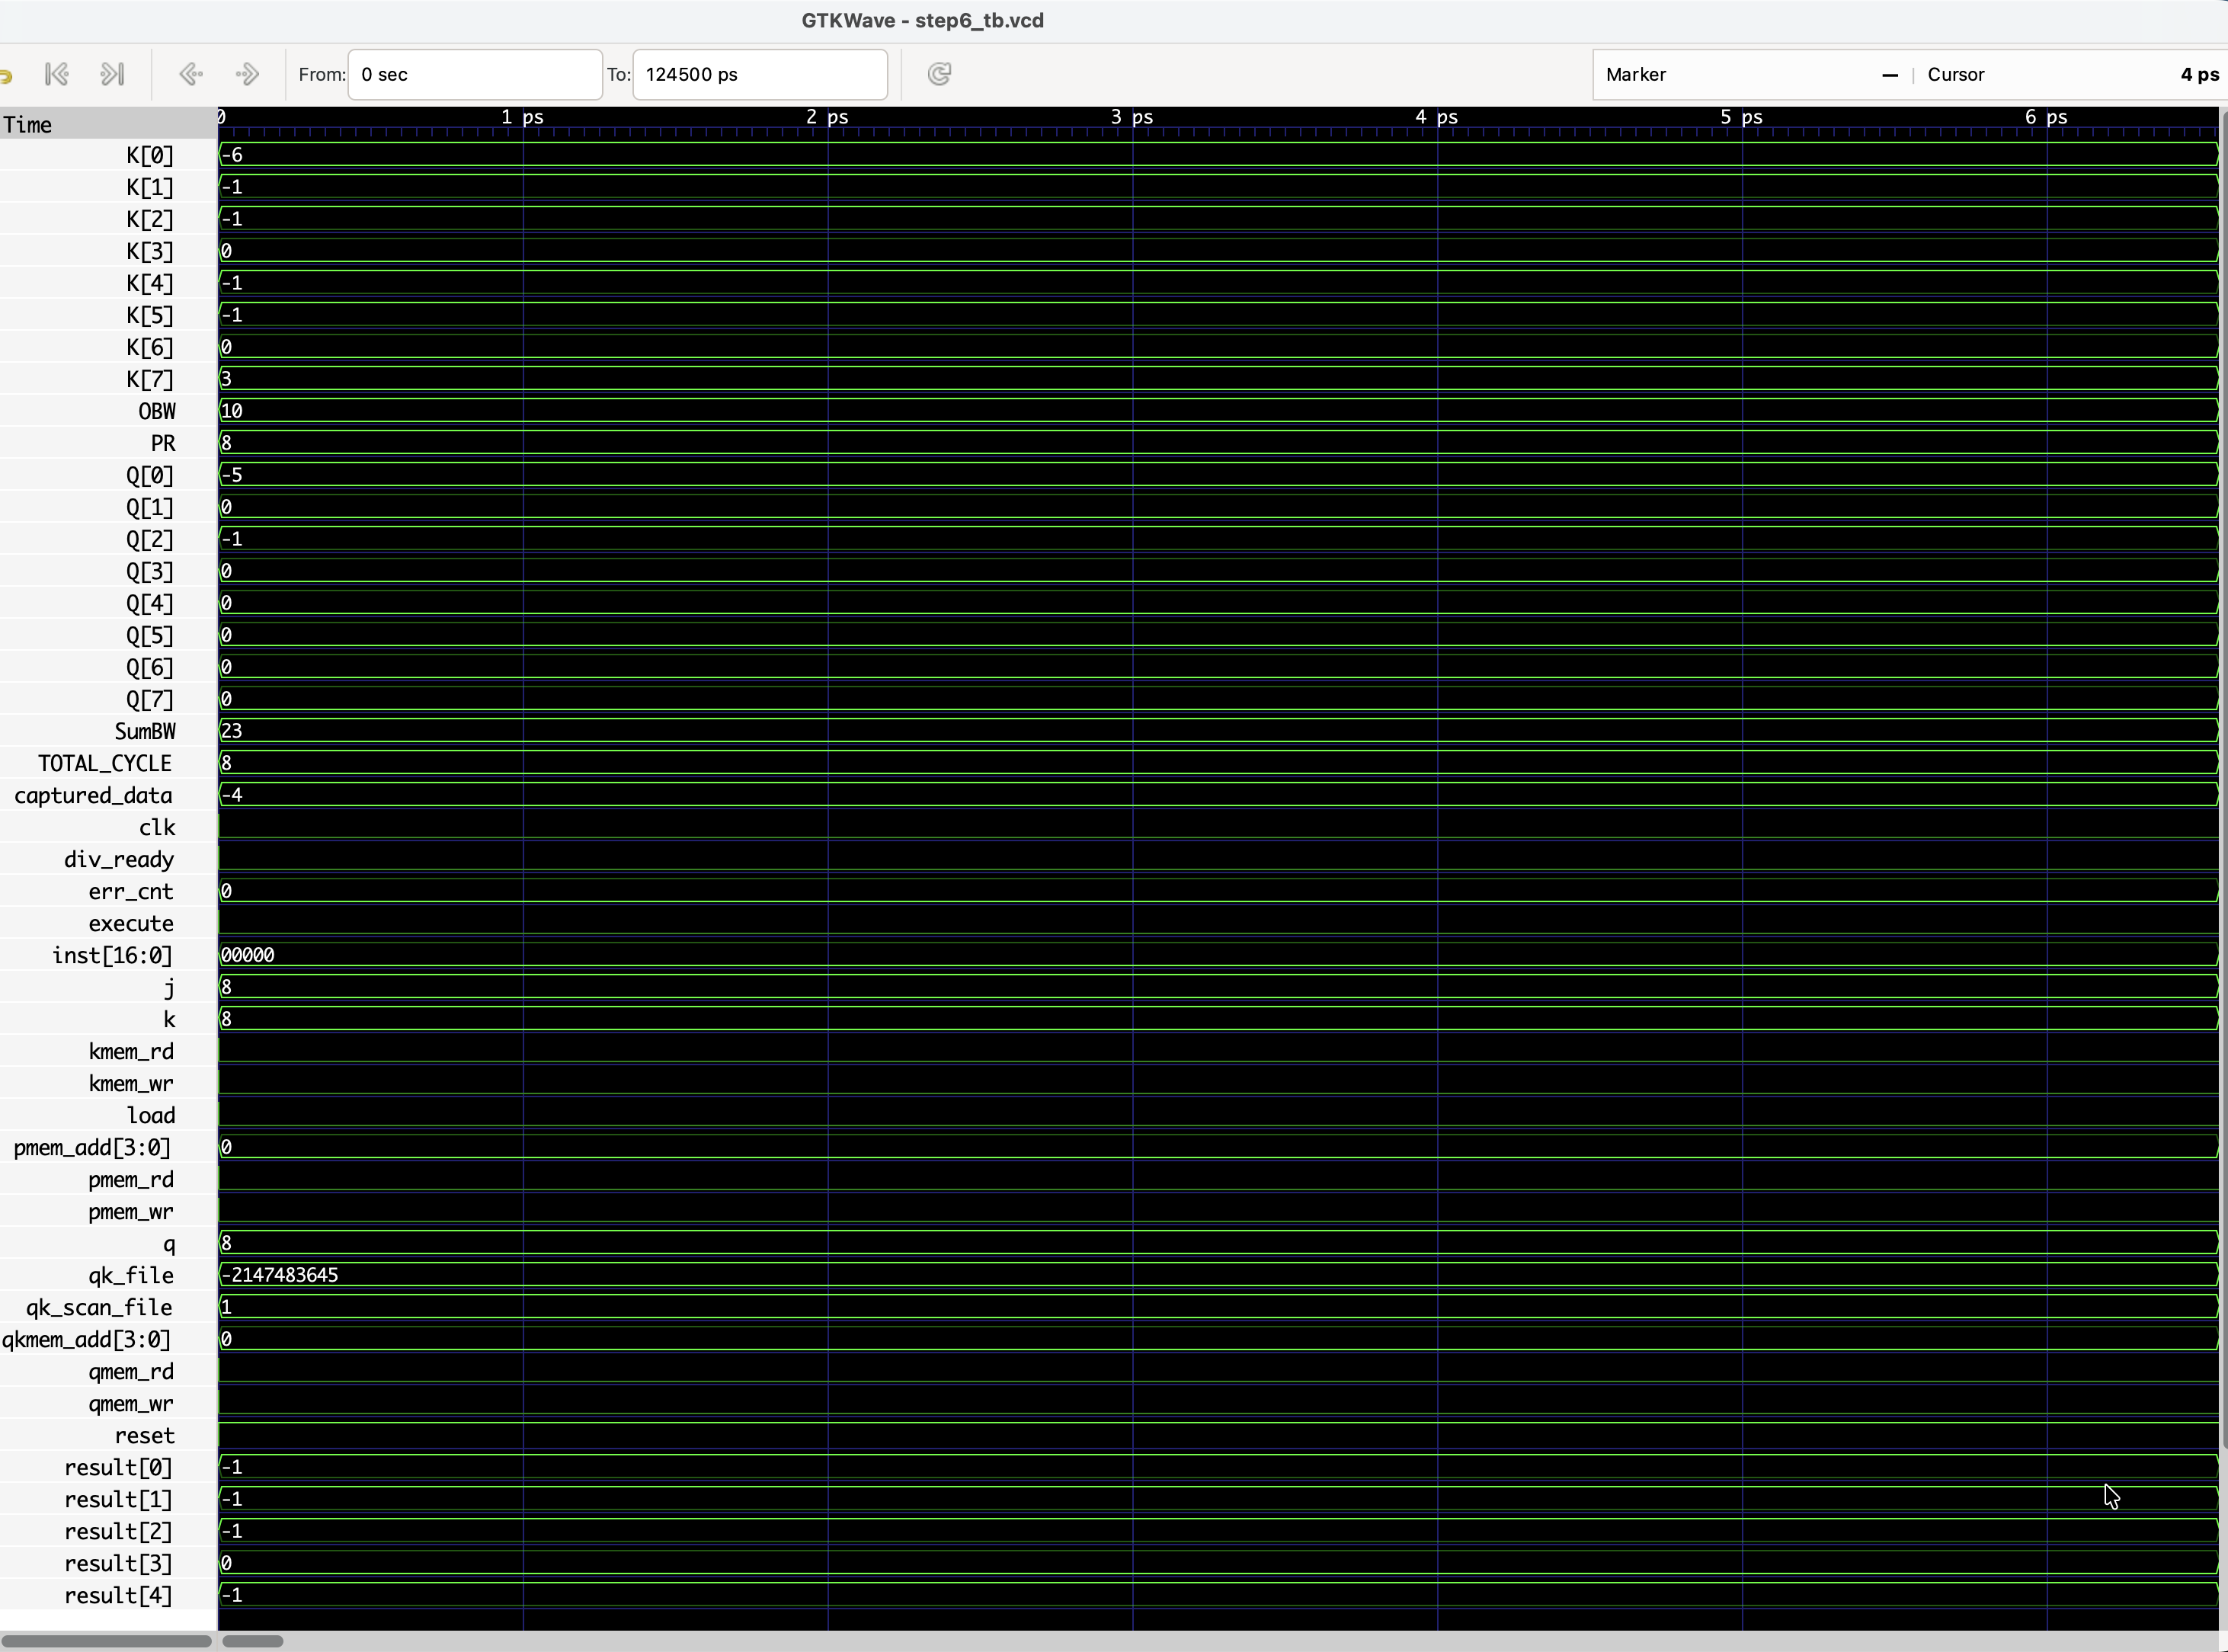
\includegraphics[width=\linewidth]{Step6_vcd.png}
    \caption{Step 6 VCD waveform}
  \end{subfigure}
  \caption{Step 6: final dual-core design with two-stage pipelined
    multiplier and sparsity controller. All tests pass.}
  \label{fig:step6}
\end{figure}

% ---------------------------------------------------------------
\section{Results and Performance Analysis}
% ---------------------------------------------------------------

\begin{table}[H]
\centering
\caption{Post-Route PnR Results (TSMC 65\,nm, 1\,GHz)}
\label{tab:results}
\small
\begin{tabular}{lcccc}
\toprule
& \textbf{Step 3} & \textbf{Step 4} &
  \textbf{Step 5} & \textbf{Step 6} \\
\midrule
Design & 1-core & 2-core & 2-core & 2-core \\
Instances & 45,972 & 167,896 & 173,920 & 173,920 \\
Area ($\mu$m$^2$) & 632,212 & 623,612 & 663,643 & 663,643 \\
WNS (ns) & +0.103 & +0.098 & +0.023 & +0.058 \\
Power (mW) & 136.4 & 428.8 & 471.7 & 471.7 \\
DRC / LVS & 0 / 0 & 0 / 0 & 0 / 0 & 0 / 0 \\
\bottomrule
\end{tabular}
\end{table}

\textbf{Timing.} All steps meet 1\,GHz with positive WNS and zero
TNS. The internal reg-to-reg critical path (\texttt{sfp\_row}
divider) maintains +0.213\,ns slack; tighter I/O paths
(+0.023\,ns in Step~5) are constrained by output delay assertions.

\textbf{Area.} Steps 5--6 add $\sim$6\% area over Step~4 due to
pipeline registers. The sparsity controller contributes $<$1\%.

\textbf{Power.} Dual-core power scales 3.1$\times$ from single-core
(136$\to$429\,mW). Element-level gating reduces MAC switching;
row-level skipping eliminates normalization for sparse rows.

\textbf{Optimization trade-off.} The two-stage multiplier adds
2 cycles of latency (4$\to$6 for PR=8) but halves per-stage
combinational depth, enabling higher frequency or lower voltage.

% ---------------------------------------------------------------
\section{Deliverables}
% ---------------------------------------------------------------

\vspace{-2pt}
\begin{table}[H]
\centering
\caption{File Paths (relative to
  \texttt{\small\textasciitilde/ece260b\_project/})}
\label{tab:deliverables}
\footnotesize
\begin{tabular}{llll}
\toprule
\textbf{Step} & \textbf{RTL} & \textbf{.enc} & \textbf{VCD} \\
\midrule
3 & \texttt{verilog/*.sv} & \texttt{pnr/step3/} &
  \texttt{verilog/step3.vcd} \\
4 & \texttt{verilog/*.sv} & \texttt{pnr/step4/} &
  \texttt{verilog/step4\_tb.vcd} \\
5 & \texttt{verilog/*.sv} & \texttt{pnr/step5/} &
  \texttt{verilog/step5\_tb.vcd} \\
6 & \texttt{verilog/*.sv} & \texttt{pnr/step6/} &
  \texttt{verilog/step6\_tb.vcd} \\
\bottomrule
\end{tabular}
\end{table}

% ---------------------------------------------------------------
\section{Conclusion}
% ---------------------------------------------------------------

This project presents a complete hardware implementation of an
attention accelerator, progressing from a single-core baseline to
a fully optimized dual-core system in TSMC 65\,nm at 1\,GHz with
zero DRC/LVS violations across all steps.

Key contributions:
\begin{enumerate}
  \item \textbf{Parallel dual-core architecture} with MUX-based
    async bus synchronizer enabling reliable CDC between 1\,GHz
    and 800\,MHz cores.
  \item \textbf{Two-stage pipelined 8-bit multiplier} that halves
    the critical multiply path by splitting at the 4-bit boundary.
  \item \textbf{Sparsity-aware computation} with element-level
    gating and row-level skipping, reducing switching activity with
    $<$1\% area overhead.
\end{enumerate}

The final design successfully balances performance (parallel
execution), efficiency (sparsity + gating), and scalability
(hierarchical design), demonstrating how hardware-software
co-design is essential for advancing next-generation AI systems.

\vspace{4pt}
\noindent\rule{\linewidth}{0.4pt}
{\footnotesize \textbf{References:}
UCSD ECE 260B Course Materials (Winter 2026).}

\end{document}
